\section{Theory}

\subsection{Background}

\begin{frame}
    \frametitle{Reinforcement Learning}

    Reinforcement learning (RL) is a paradigm for learning mappings from observations to actions.
    
    Partially observable Markov decision process (POMDP):

    \begin{itemize}
        \item Agent interacts with environment over discrete time steps \(t = 0, 1, 2\dots\)
        \item Takes action \(a_t\) in state \(s_t\)
        \item Perceives observation \(o_t\) 
        \item New state \(s_{t+1}\)
    \end{itemize}

    \begin{figure}
        \centering
        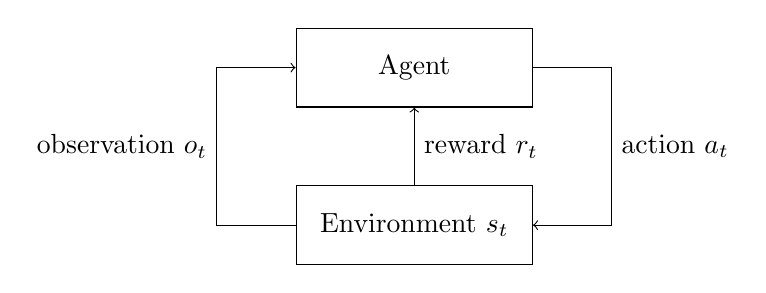
\begin{tikzpicture}[node distance=2cm]
    \tikzstyle{block} = [rectangle,minimum width=3cm,minimum height=1cm,text centered,draw=black,fill=white]
    \node (agent)[block]{Agent};
    \node (environment)[block,below of=agent]{Environment \(s_t\)};
    \draw [->] (agent.east) -- ++(1cm,0) -- node [anchor=west]{action \(a_t\)} ++(0,-2cm) -- (environment.east);
    \draw [->] (environment.north) -- node [anchor=west]{reward \(r_t\)} (agent.south);
    \draw [->] (environment.west) -- ++(-1cm,0) -- node [anchor=east]{observation \(o_t\)} ++(0,+2cm) -- (agent.west);
\end{tikzpicture}
    \end{figure}
\end{frame}

\subsection{Related Work}

\begin{frame}
    \frametitle{Search with Reinforcement Learning}

    \dots
\end{frame}